% Template for ICIP-2015 paper; to be used with:
%          spconf.sty  - ICASSP/ICIP LaTeX style file, and
%          IEEEbib.bst - IEEE bibliography style file.
% --------------------------------------------------------------------------
\documentclass{article}
\usepackage{spconf,amsmath,graphicx}
\usepackage[utf8]{inputenc} % Suporte para acentuação sem necessidade dos comandos especiais.
\usepackage{amsmath,epsfig}
\usepackage[portuguese,algoruled,longend]{algorithm2e}
\usepackage{multirow}
\usepackage{MnSymbol}
\usepackage{wasysym}
\usepackage[table,xcdraw]{xcolor}
\usepackage[brazilian]{babel}
\usepackage{url}
\usepackage{float}
\usepackage[inline]{enumitem}
\usepackage{enumerate}
\usepackage{soul,framed} %,caption
\colorlet{shadecolor}{yellow}

% Template includegraphics
% \begin{figure}[H]
% 	\begin{center}
% 		\label{fig:11}
% 		\includegraphics[width=2.5in]{Figures/S02_Grafico_Ajustado.png}
% 		\caption{Gráficos da Situação 03 Ajustados}
% 	\end{center}
% \end{figure}

% Example definitions.
% -------------------
\def\x{{\mathbf x}}
\def\L{{\cal L}}

% Title.
% ------
\title{Processamento de Sinais Biológicos - Estimação da DEP em sinais de eletrocardiograma (ECG)}
%
% Single address.
% ---------------
\name{Davi de Alencar Mendes - 16/0026415}
\address{Engenharia Eletrônica, UnB-FGA, Brasília, Brasil}


\begin{document}

\maketitle

\begin{abstract}
O presente trabalho explora a estimação de DEP em sinais de ECG. São considerados dois cenários:
\begin{enumerate*}[label=(\roman*)]
		\item estimação da DEP para versões janeladas do sinal;
		\item estimação da DEP para os complexos QRS do sinal.
\end{enumerate*}
O desenvolvimento é realizado com auxílio de ferramentas computacionais, em especial MATLAB, e com sinais reais de ECG no qual não há segmentos com anomalias (arritmias, etc). Finalmente, o trabalho tem como finalidade expor os resultados obtidos e os métodos utilizados.
\end{abstract}


\section{Estimação da DEP para versões janeladas em sinais de ECG}
Por se tratar de um sinal ciclo periódico, os sinais de ECG apresentam um período relativamente controlado embora não seja constante ao longo do tempo. Nesse sentido, a estimação da DEP ao longo de ciclos cardíacos provê informações de grande valia para o desenvolvimento de algoritmos para detecção de características de interesse do sinal que estão localizadas em bandas diferentes de frequência.

\subsection{Metodologia}
Inicialmente, define-se uma duração de uma janela para qual será realizada o recorte do sinal. O sinal analisado é preenchido com zeros caso seu tamanho não seja múltiplo do tamanho escolhido para a janela. Ressalta-se que não há sobreposição entre as janelas e que para o trabalho realizado foi escolhido uma janela retangular. Posteriormente, é calculado o periodograma para cada uma das janelas e uma média de todas as janelas calculadas torna-se a estimativa para a DEP das realizações observadas.

\subsection{Resultados}

\begin{figure}[H]
	\begin{center}
		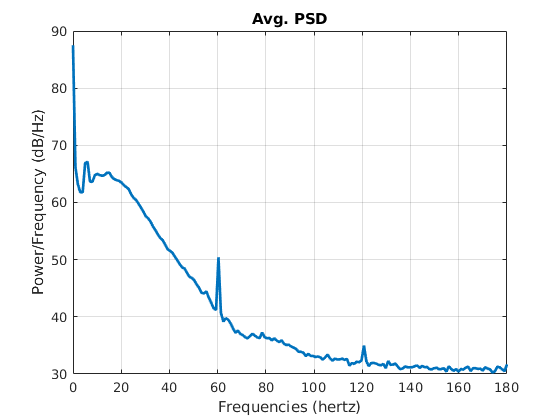
\includegraphics[width=2.5in]{Figures/avg_psd.png}
		\caption{DEP média para as janelas do sinal utilizado}
		\label{fig:1avg}
	\end{center}
\end{figure}

\begin{figure}[H]
	\begin{center}
		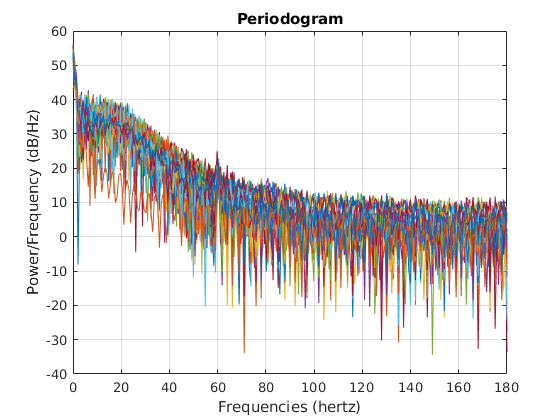
\includegraphics[width=2.5in]{Figures/periodogram_all.png}
		\caption{Sobreposição dos Periodogramas para cada janela do sinal utilizado}
		\label{fig:1all}
	\end{center}
\end{figure}

\section{Estimação da DEP para complexo QRS}
A estimação da DEP para o complexo QRS requer a extração dessas características temporais do sinal em análise. Para tal, apresenta-se uma abordagem para extração de complexo QRS baseada em operações de filtragem linear, filtragem derivativa seguida de operações não lineares para extrair as informações desejadas do sinal.

\subsection{Metodologia}
A extração dos pontos Q \& S foi realizada após a extração dos picos R, considerando os pontos Q \& S como os mínimos locais entre cada um dos picos R. Para localizar os picos R foi desenvolvida uma função chamada \textit{rwave\_detect}. O procedimento para localizar os picos R consiste em:
\begin{itemize}
	\item Filtrar o sinal em uma banda de frequência (0.5-60Hz) usando filtros \textit{zero-phase};
	\item Aplicar um filtro derivativo do tipo FIR;
	\item Normalizar os valores obtidos pelo máximo absoluto;
	\item Elevar ao quadrado para ressaltar conteúdos de alta frequência presentes no sinal;
	\item Filtrar o sinal com uma média móvel para uniformizar os picos presentes;
	\item Localizar picos por limiarização e distância mínima entre picos de 200ms.
\end{itemize}

\subsection{Resultados}
Os resultados obtidos são, de maneira geral, satisfatórios porém o algoritmo não é robusto para adequar-se a sinais com grandes deformações ou anomalias. Após marcação de todos os pontos de interesse foi avaliada a DEP (figura ~\ref{fig:2dep}) para os complexos QRS concatenados lado-a-lado (figura ~\ref{fig:2qrs}).

\begin{figure}[H]
	\begin{center}
		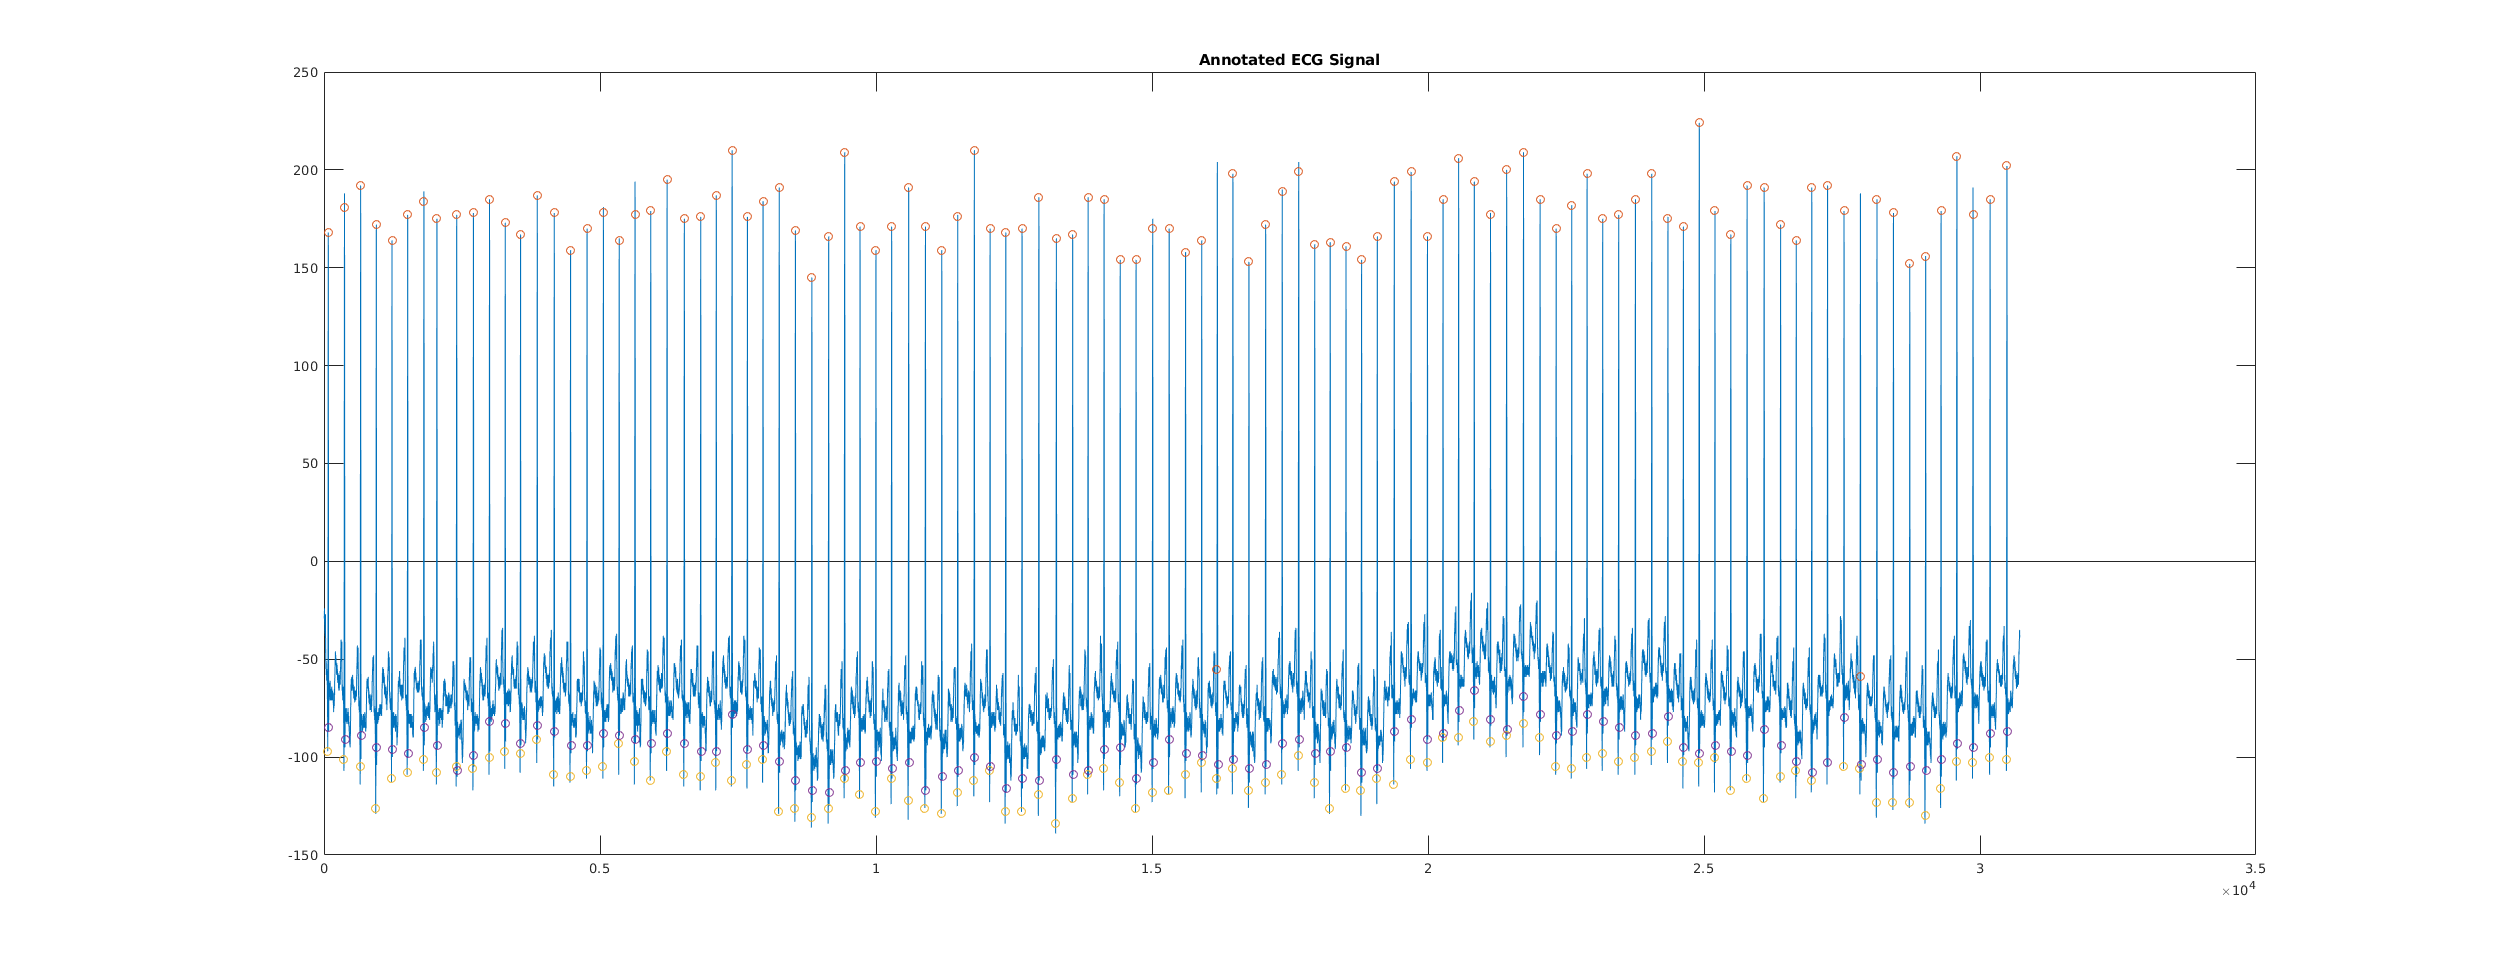
\includegraphics[scale=0.11]{Figures/ann_ecg.png}
		\caption{Sinal de ECG com anotações}
		\label{fig:2ann}
	\end{center}
\end{figure}

\begin{figure}[H]
	\begin{center}
		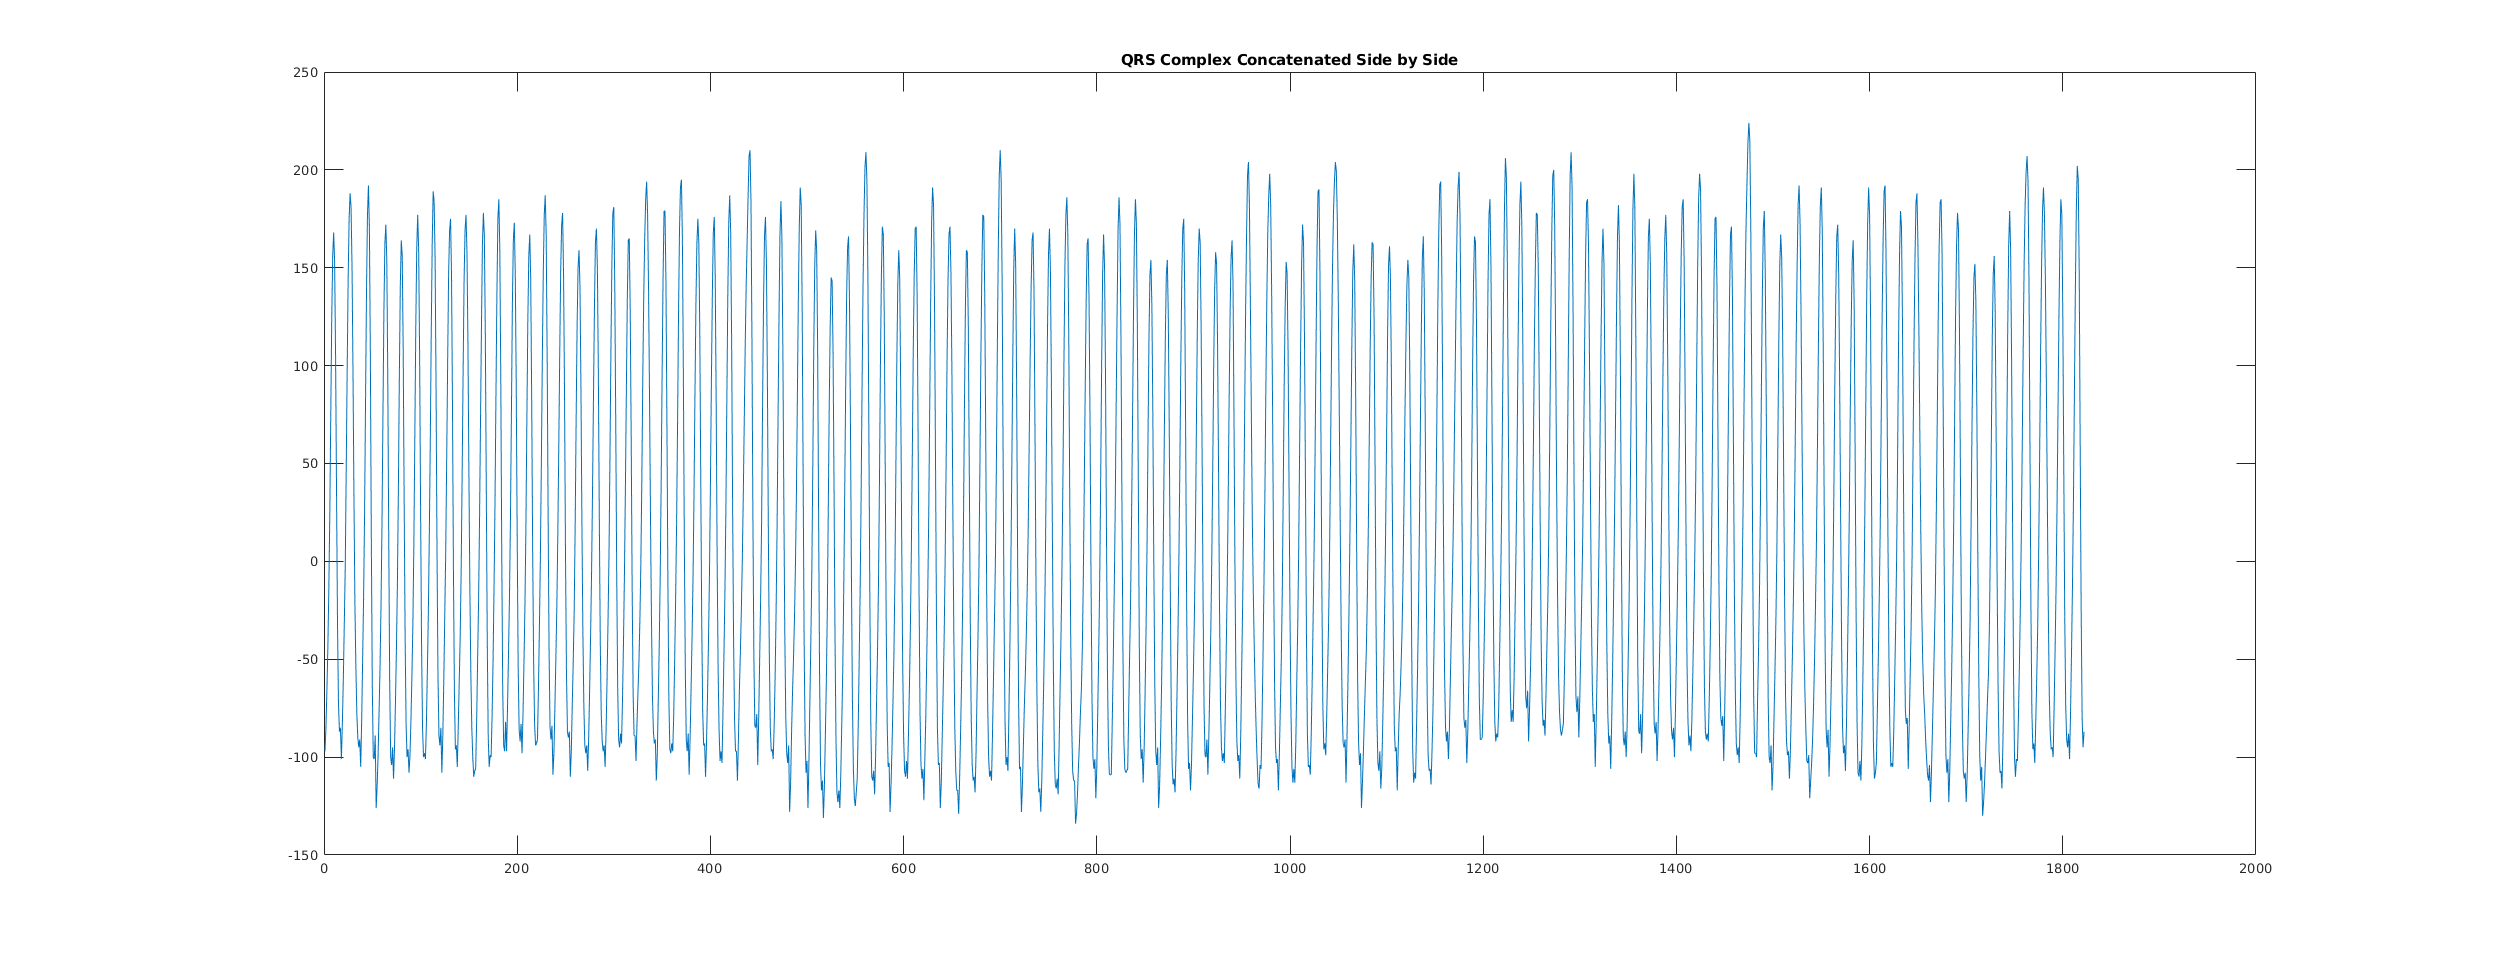
\includegraphics[scale=0.11]{Figures/qrs_sideside.png}
		\caption{Complexos QRS extraídos}
		\label{fig:2qrs}
	\end{center}
\end{figure}

\begin{figure}[H]
	\begin{center}
		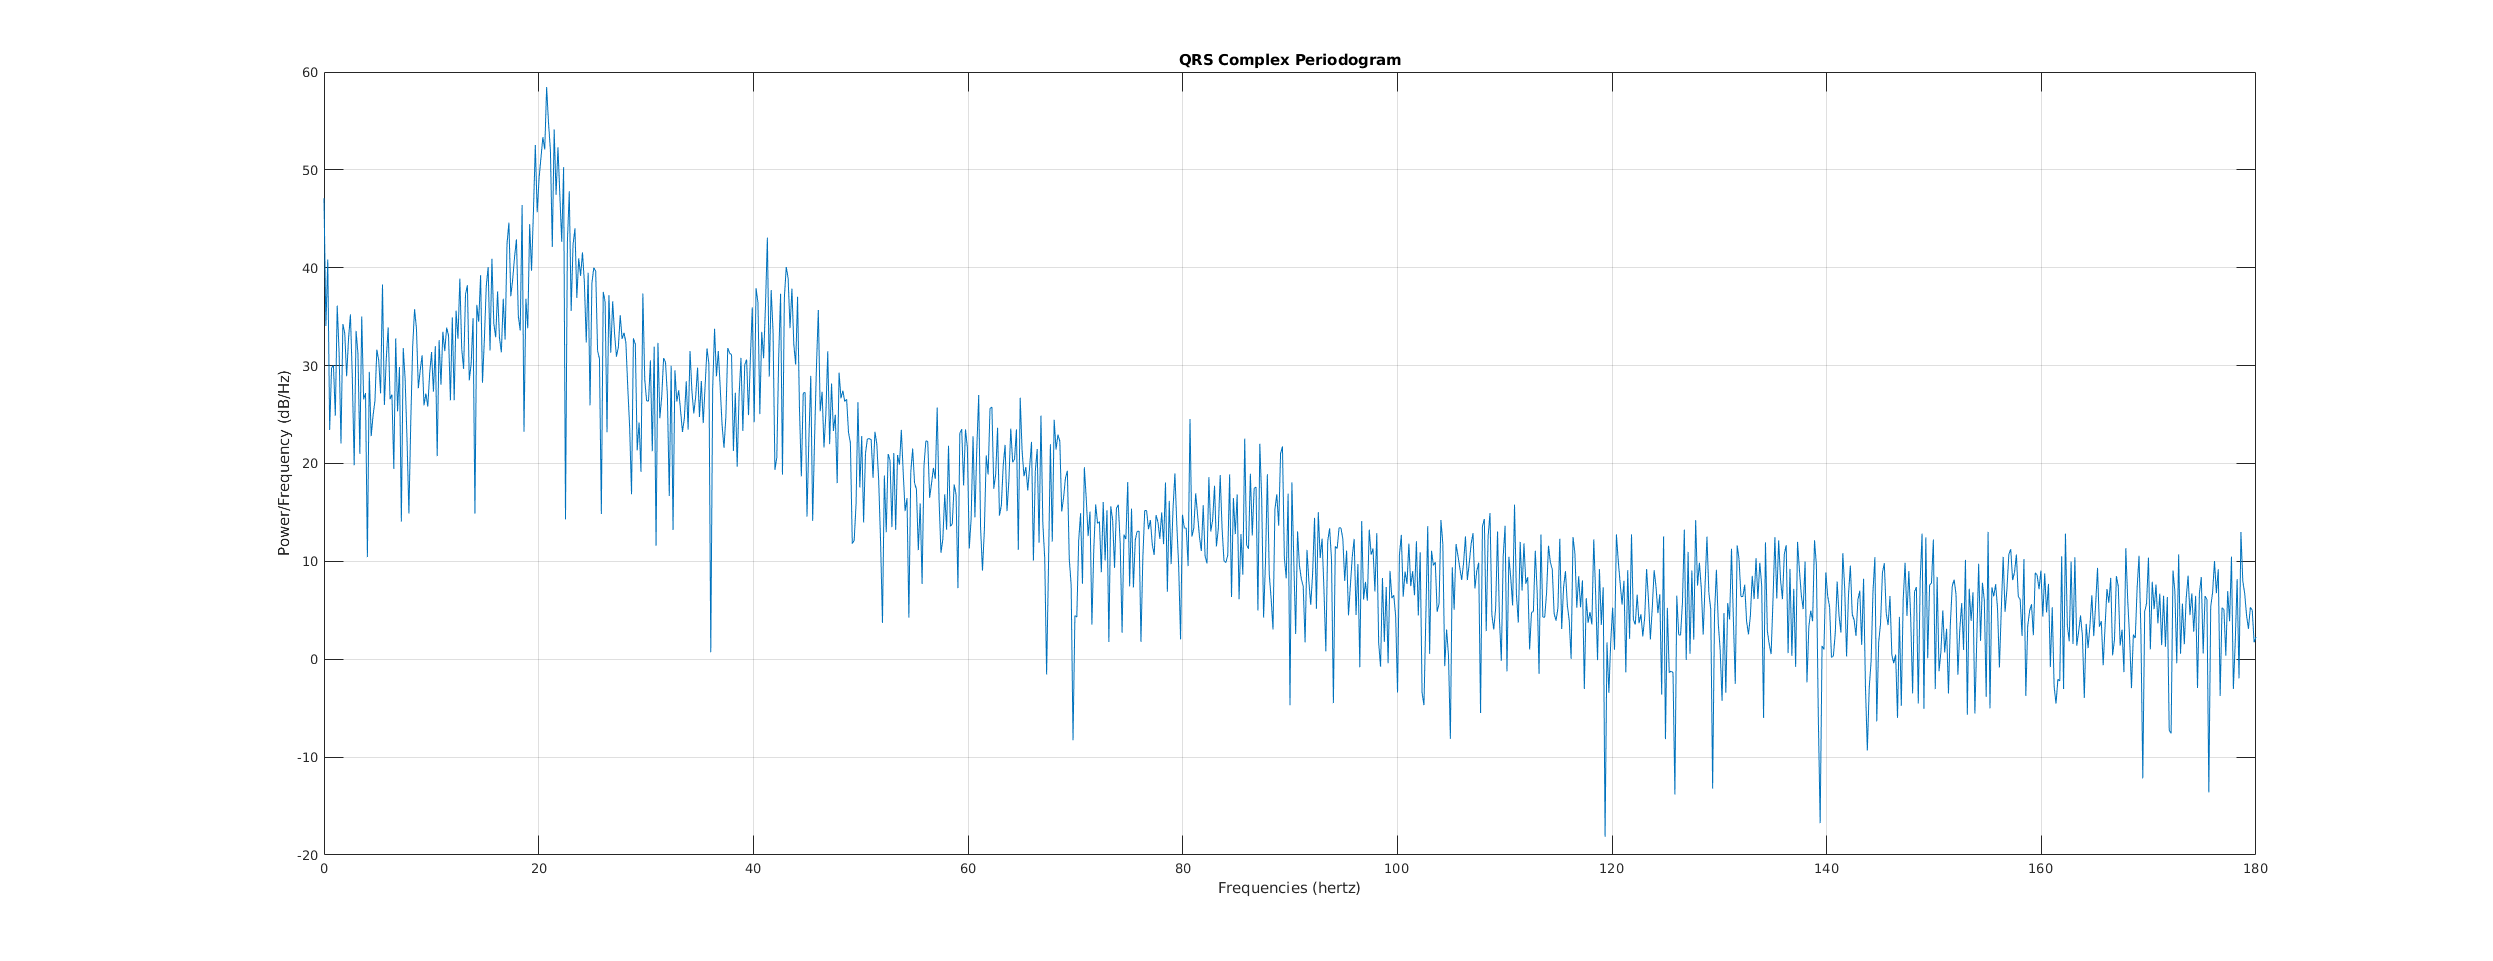
\includegraphics[scale=0.11]{Figures/dep_qrs.png}
		\caption{DEP dos complexos QRS extraídos}
		\label{fig:2dep}
	\end{center}
\end{figure}

% -------------------------------------------------------------------------
% \begin{thebibliography}{1}

% \bibitem{ref:gonzalez}
% Gonzalez, Rafael C., author. Digital image processing / Rafael C. Gonzalez, University of Tennessee, Richard E. Woods, Interapptics. New York, NY : Pearson, [2018]

% \end{thebibliography}
\end{document}
